This chapter covers relevant concepts for $0 \nu \beta \beta$ decay searches. It begins with an introduction to the Standard Model, explaining why its minimal formulation cannot account for neutrino masses. It then presents evidence that neutrinos can change flavor during propagation, implying that neutrinos can not be massless. 
Next, it discusses two different mechanisms for generating neutrino masses, considering neutrinos as Dirac or Majorana particles. After a brief theoretical introduction to $0 \nu \beta \beta$ decay, several experimental results are discussed. 
The chapter concludes with the introduction of the next-generation $0 \nu \beta \beta$ decay experiments.

\subsection{Neutrinos in the Standard Model of particle physics}
The last few centuries of physics research have concluded that there are four fundamental interactions in nature: gravity, described by the theory of general relativity, and the electromagnetic, weak, and strong interactions. The latter three are unified in the framework of the Standard Model of particle physics (SM), a gauge quantum field theory in which particles arise as quantized excitations of the underlying fields~\cite{peskin_introduction_2019}. 

The total gauge symmetry of the SM is $SU(3)_C \times SU(2)_L \times U(1)_Y$. The $SU(3)$ component of the SM is related to quantum chromodynamics, the theory of the strong force. 
It describes how quarks, carrying color charge, are confined to form hadrons. The remaining part of the SM gauge symmetry corresponds to the unification of the electromagnetic and the weak interaction. The $L$ indicates that the weak interaction couples to left-handed particles, as only left-handed fermions (and right-handed anti-fermions) participate in weak-isospin doublets. The group $U(1)_Y$ is associated with the weak hypercharge $Y$. 

In the SM, there are three generations of leptons: The three charged leptons $e$, $\mu$, and $\tau$ and their corresponding neutrinos ($\nu_e, \nu_\mu, \nu_\tau$). These leptons are grouped into $SU(2)_L$ doublets for the left-handed components. Usually, $l_L$ denotes an unspecified $SU(2)_L$ doublet while $l_R$ refers to the corresponding right-handed singlet, which does not participate in weak-isospin interactions:

\begin{equation} 
\label{eq:su2_leptonic_doublets}
l_L = 
	\begin{pmatrix} \nu_{\text{l}} \\ \text{l} \end{pmatrix}, \; 
    l_R = \text{l}_R \,.
\end{equation}

\noindent Here, $\text{l}$ represents one of the charged leptons and $\nu_l$ its corresponding neutrino.
The four generators of the electroweak gauge symmetry, corresponding to $SU(2)_L$ and $U(1)_Y$, do not directly correspond to physical particles. Instead, specific linear combinations of these generators give rise to the physical gauge bosons of the weak and electromagnetic interactions. 
Two $SU(2)_L$ gauge bosons form the charged weak gauge bosons $W_{\mu}^{\pm}$, which mediate charged current (CC) interactions such as $\beta$-decays. The Lagrangian is given in~\refeq{eq:Lagr_weak_CC}, where $\gamma^{\mu}$ represents the Dirac matrices and $g$ denotes the weak coupling constant. The notation $\overline{\nu_{l, L}} = (\nu_{l, L})^\dagger \gamma^0$ and $\overline{l^{-}_{L}} = (l_L)^\dagger \gamma^0$ denotes the Dirac adjoint of the left-handed neutrino and lepton fields, respectively.

\begin{equation}
\label{eq:Lagr_weak_CC}
    \Lagr_{CC} = - \frac{g}{\sqrt{2}} \sum_l \left( \overline{\nu_{l, L}} \gamma^{\mu} l^{-}_{L} W^{+}_{\mu} + \overline{l^{-}_{L}} \gamma^{\mu} \nu_{l, L} W^{-}_{\mu} \right) \,.
\end{equation}

The remaining $SU(2)_L$ gauge boson, $W^3_{\mu}$ mixes with the $U(1)_Y$ gauge boson to form the electrically neutral $Z_{\mu}$ boson and the photon, $A_{\mu}$, according to the following relation

\begin{equation}
\label{eq:weak_mixing}
\begin{pmatrix}
    Z^0_{\mu} \\ A_{\mu}
\end{pmatrix}
= \begin{pmatrix}
    \cos \theta_W \; - \sin \theta_W \\
    \sin \theta_W \; + \cos \theta_W 
\end{pmatrix}
\begin{pmatrix}
    W^3_{\mu} \\ B_{\mu}
\end{pmatrix} \,,
\end{equation}

\noindent where $W^3_{\mu}$ is the third gauge boson of the $SU(2)_L$ group, $B_{\mu}$ is the gauge boson of the $U(1)_Y$ group, and $\theta_W$ is the weak mixing angle~\cite{weinberg_quantum_1995, navas_review_2024}. 
The $Z^0_{\mu}$ boson mediates weak neutral current (NC) interactions, with the corresponding Lagrangian given in equation~\refeq{eq:Lagr_weak_NC}. Weak NC interactions depend on the weak hypercharge and therefore couple also to right-handed fermions (and left-handed anti-fermions). 
However, in the minimal Standard Model, right-handed neutrinos do not exist, as they are completely uncharged under the gauge interactions.

\begin{equation}
\label{eq:Lagr_weak_NC}
    \Lagr_{NC} = - \frac{g}{2 \cos \theta_W} \sum_l \overline{\nu_{l, L}} \gamma^{\mu} \nu_{l, L} Z^0_{\mu} \,.
\end{equation}


In the unbroken electroweak theory, all gauge bosons and fermions are massless. However, the introduction of the Higgs field $\phi$, a complex scalar doublet, leads to spontaneous symmetry breaking of the $SU(2)_L \times U(1)_Y$ gauge symmetry. This mechanism generates masses for $W^{\pm}$ and $Z^{0}$ bosons, while leaving the photon massless. 
When the Higgs field acquires a non-zero vacuum expectation value $\langle\phi \rangle  = \frac{1}{\sqrt{2}} \begin{pmatrix} 0 \\ v \end{pmatrix}$, the symmetry is spontaneously broken and the weak gauge bosons acquire mass. The mass of the charged weak bosons is given by

\begin{equation}
\label{eq:W_boson_mass}
    m_W = \frac{1}{2} g v \,,
\end{equation}

\noindent where $g$ is weak coupling constant and $v \approx 246$~GeV is the Higgs vacuum expectation value~\cite{navas_review_2024}. 
At energies much lower than $m_W$, the exchange of a virtual $W$ boson can be approximated by a point-like interaction. The corresponding coupling strength is the Fermi constant $G_F$, defined as

\begin{equation}
\label{eq:Fermi_constant}
    G_F = \frac{\sqrt{2}}{8} \frac{g^2}{m_W^2} \approx 10^{-5} \mathrm{GeV}^{-2} \,.
\end{equation}

This low-energy limit reproduces the structure of Fermi's original theory of beta decay, in which weak interactions are modeled as point-like four-fermion interactions with a universal coupling constant~\cite{peskin_introduction_2019}.

Fermion masses are generated through interactions with the Higgs field via the Yukawa coupling. The Yukawa coupling for the electron is described by equation~\refeq{eq:Lagr_Yukawa_e}, where the Hermitian conjugate of the Higgs field is indicated by $\phi^\dagger$ and the Yukawa coupling constant for the electron by $Y_e$~\cite{peskin_introduction_2019}:

\begin{equation} 
\label{eq:Lagr_Yukawa_e}
		\Lagr_Y^e = -Y_e \left( \overline{l_L} \phi l_R + \overline{l_R} \phi^{\dagger} l_L \right) \,.
\end{equation}

When the Higgs field acquires a non-zero vacuum expectation value, the symmetry is spontaneously broken and the electron acquires a mass term proportional to both the Yukawa coupling constant and the vacuum expectation value of the Higgs field~\cite{bilenkij_introduction_2018, navas_review_2024}:

\begin{equation} 
\label{eq:electron_mass}
		m_e = Y_e \cdot \frac{v}{\sqrt{2}} \,.
\end{equation}


This mechanism applies analogously to other fermions, with each particle's mass depending on its specific Yukawa coupling constant. However, since right-handed neutrinos are completely uncharged in the electroweak theory, it is not possible to construct a Yukawa term analogous to~\refeq{eq:Lagr_Yukawa_e}. As a result, the Standard Model predicts that neutrinos are massless~\cite{navas_review_2024}. 

\subsection{Neutrino oscillation}

Already in 1967, Pontecorvo proposed a mechanism where lepton flavor is not conserved during neutrino propagation, leading to the phenomenon known as neutrino oscillation~\cite{pontecorvo_neutrino_1968}. Since then, several experiments have observed deficits in neutrino fluxes from the sun (solar neutrinos), the atmosphere (atmospheric neutrinos), nuclear reactors and particle accelerators, providing strong evidence for neutrino oscillation. In addition to these disappearance signals, later experiments such as OPERA and NOvA have directly observed the appearance of different neutrino flavors, confirming the oscillation mechanism through both disappearance and appearance channels~\cite{opera_neutrino_2019, Acero_nova_2022}.

Atmospheric neutrinos are produced in collisions of cosmic rays with nuclei from the upper atmosphere. The flux is dominated by leptonic pion decays, yielding an expected ratio of:

\begin{equation}
\label{eq:Neurino_flux_ratio}
    \frac{\Phi_{\nu_\mu} + \Phi_{\overline{\nu}_{\mu}}}{\Phi_{\nu_e} + \Phi_{\overline{\nu}_e}} \approx 2 \,.
\end{equation}

The first precise measurement for neutrino oscillation was presented in 1998 by the Super-Kamiokande experiment, a 50 kiloton water Cherenkov detector equipped with over 11'000 photomultiplier tubes (PMTs), located 1000 meters below ground in Japan. Neutrinos are detected via charged current neutrino scattering and subsequent Cherenkov radiation of the leptons~\cite{super-kamiokande_collaboration_evidence_1998}. 
Super-Kamiokande also detected a smaller than expected solar $\nu_e$ flux originating from different nuclear fusion processes, indicating neutrino oscillation in solar neutrinos~\cite{super-kamiokande_collaboration_solar_2001}. This discrepancy between theoretically predicted and experimentally observed $\nu_e$ flux is called the solar neutrino problem. It was solved by the Sudbury Neutrino Observatory (SNO), which provided a crucial breakthrough by detecting both charged-current and neutral-current interactions. By comparing these interaction rates, SNO showed that the total flux of solar neutrinos agreed with theoretical predictions from the Standard Solar Model, but a substantial fraction had transformed into $\nu_\mu$ and $\nu_\tau$ flavors~\cite{SNO_solar_neutrino_2022}.

In general, a neutrino $\nu_{\alpha}$ is produced in a definitive flavor eigenstate ($\nu_e$, $\nu_{\mu}$, $\nu_{\tau}$) via the weak interaction. This neutrino then propagates through spacetime as a linear superposition of the three mass eigenstates ($\nu_1$, $\nu_2$, $\nu_3$), which are the actual fundamental particles. When a neutrino is later detected, it is again projected onto a specific flavor eigenstate, which may differ from its original production state, leading to the possibility of flavor transitions~\cite{thomson_modern_2013, zuber_neutrino_2020}. 
The flavor eigenstates $\nu_{\alpha}$ and mass eigenstates $\nu_i$ are connected through the unitary Pontecorvo–Maki–Nakagawa–Sakata (PMNS) matrix $\mathcal{U}$:

\begin{equation}
\label{eq:neutrino_eigenstates}
	\ket{\nu_{\alpha}}= \sum_i^3 \mathcal{U} \ket{\nu_i}\,.
\end{equation}

This mixing leads to the phenomenon of neutrino oscillation, where a neutrino can change its flavor as it propagates through space. 
The PMNS matrix is typically parametrized by three mixing angles ($\theta_{12}$, $\theta_{13}$, $\theta_{23}$) and a complex phase $\delta$, which can lead to charge-parity (CP) violation in the lepton sector. CP violation in neutrino oscillations is a key area of current research, as it could provide insights into the matter-antimatter asymmetry of the universe. The parametrization, shown in~\refeq{eq:PMNS_matrix}, uses the shorthand $s_{ij} = \sin \theta_{ij}$ and $c_{ij} = \cos\theta_{ij}$. Although the full PMNS matrix contains 18 real parameters, only four of them are physically observable in neutrino oscillation experiments~\cite{navas_review_2024, thomson_modern_2013}.


\begin{equation}
\label{eq:PMNS_matrix}
	\mathcal{U} = \begin{pmatrix} 
	c_{12} \, c_{13} & s_{12}\, c_{13} & s_{13} \, e^{-i \delta_{CP}} \\ 
	-s_{12} \, c_{23} - c_{12} \, s_{13} \, s_{23} \, e^{i \delta_{CP}} & c_{12} \, c_{23} - s_{12} \, s_{13} \, s_{23} \, e^{i \delta_{CP}} & c_{13} \, s_{23} \\
	s_{12} \, s_{23} - c_{12} \, s_{13} \, c_{23} \, e^{i \delta_{CP}} & -c_{12} \, s_{23} - s_{12} \, s_{13} \, c_{23} \, e^{i \delta_{CP}} & c_{13} \, c_{23} \\ \end{pmatrix} 
\end{equation}

\noindent For two-flavor mixing, the probability of neutrino oscillation is given by:

\begin{equation} 
\label{eq:neutrino_oscillation_prob}
    P_{\alpha \to \beta}(t) = \abs{\bra{\nu_{\beta}} \ket{\nu_{\alpha}(t)}}^2 = \sin^2 \left( 2 \theta \right) \cdot  \sin^2 \left( \Delta m^2_{ij} \cdot \frac{L}{4E} \right) \,,
\end{equation}

\noindent where, $\Delta m^2_{ij} = m^2_i - m^2_j$ is the squared mass difference between mass eigenstates $i$ and $j$, $L$ the distance between source and detection, and $E$ the neutrino energy~\cite{zuber_neutrino_2020}. 
Equation~\refeq{eq:neutrino_oscillation_prob} illustrates that the oscillation probability depends on the squared mass differences, not the absolute masses. Consequently, neutrino oscillations require $\Delta m^2_{ij} \neq 0$, and oscillation experiments cannot determine the absolute neutrino mass scale. 
The mixing angle $\theta$ in the two-flavor oscillation probability arises from the underlying unitary transformation that relates flavor and mass eigenstates, analogous to equation~\refeq{eq:neutrino_eigenstates}. In the absence of CP violation, this transformation reduces to a real, orthogonal matrix with a single parameter (an element of $SO(2)$). The angle $\theta$ determines the amplitude of the oscillation probability~\cite{zuber_neutrino_2020}. 

While the two-flavor approximation is useful for illustrative purposes, a complete description of neutrino oscillations involves three-flavor mixing, incorporating all three mass eigenstates and the full PMNS matrix. This more general framework leads to a richer phenomenology, including interference effects between multiple oscillation modes and potential CP-violating effects. 


\subsection{Dirac and Majorana neutrinos}

The discovery of neutrino oscillation -- and therefore the existence of non-zero masses for the neutrinos -- raises the fundamental question of how neutrinos acquire mass. Two popular mechanisms exist to generate neutrino mass terms:
If neutrinos are Dirac particles, masses can be generated by introducing right-handed neutrinos, which are often called sterile because they do not participate in SM interactions. This allows the construction of a Yukawa coupling term analogous to that of the electron, as shown in equation~\refeq{eq:Lagr_Yukawa_e}, leading to a mass term:

\begin{equation}
\label{eq:Yukawa_neutrino}
    m_{\nu} = \frac{Y_{\nu} v}{\sqrt{2}} \,.
\end{equation}

However, the SM offers no satisfactory explanation for why the neutrino Yukawa couplings (and therefore the neutrino masses) are many orders of magnitude smaller than those of other fermions~\cite{giunti_fundamentals_2007}. 

The second possibility is that neutrinos are Majorana particles, meaning they are their own antiparticles: $ \nu^C = \nu$. In this case, right-handed neutrinos are not required, since the charge-conjugated left-handed neutrino field $\nu^C_L$ transforms as a right-handed field. 
The Majorana condition for a general field is expressed as

\begin{equation} 
\label{eq:majorana_condition1}
    \psi = C \overline{\psi}^T \,,
\end{equation}

\noindent where $C$ is the charge-conjugation operator and $\overline{\psi}^T = (\psi^\dagger \gamma^0)^T$ is the transposed Dirac adjoint of $\psi$. 
If neutrinos are Majorana particles, the total lepton number $L = L_e + L_{\mu} + L_{\tau}$ is not conserved, violating a fundamental symmetry of the Standard Model. This has profound implications for physics beyond the Standard Model, including potential mechanisms such as leptogenesis, which could potentially explain the matter-antimatter asymmetry of the universe~\cite{giunti_fundamentals_2007}. 
Moreover, Majorana neutrinos introduce two additional CP-violating phases, known as Majorana phases, to the PMNS matrix. The full Majorana mixing matrix can be written as

\begin{equation}
\label{eq:Majorana_PMNS_matrix}
    \mathcal{U}^M = \mathcal{U}^D \cdot \text{diag}(1, e^{i \alpha}, e^{i \beta}) \,, 
\end{equation}

\noindent where $\mathcal{U}^D$ is the standard Dirac neutrino mixing matrix, and $\alpha$, $\beta$ are Majorana phases~\cite{zuber_neutrino_2020}. These phases, however, do not affect neutrino oscillation probabilities since they cancel out in the oscillation formula (equation~\refeq{eq:neutrino_oscillation_prob}).
The Majorana mass term for the neutrino is given by

\begin{equation} 
\label{eq:lagr_neutrino_majorana_mass}
    \Lagr^M_{mass} = - \frac{1}{2} m \left( \overline{\nu^C_L} \nu_L + \overline{\nu_L} \nu^C_L \right) \,,
\end{equation}

\noindent where $m$ is the Majorana mass term. 

While this discussion assumes three active neutrino species, extensions with sterile neutrinos are under investigation but are not addressed here. 
A compelling framework that incorporates both Dirac and Majorana mass terms is the Type-1 see-saw mechanism~\cite{yanagida_seesaw_1980}. In this scenario, heavy right-handed neutrino fields are introduced as Standard Model singlets. These fields allow for both Dirac mass terms $m_D$, arising from the Higgs mechanism as in the Dirac sense, and a large Majorana mass term $M_R$ for the right-handed neutrinos. The resulting mass Lagrangian takes the form:

\begin{equation} 
\label{eq:lagr_seesaw_mass}
    \Lagr_{mass} = - \frac{1}{2} \left( \overline{\nu_L} \; \overline{(\nu_R)^C} \right)  \begin{pmatrix}
        0 & m_D \\ 
        m_D^T & M_R
    \end{pmatrix}
    \begin{pmatrix}
        (\nu_L)^C \\ \nu_R
    \end{pmatrix} + \mathrm{h.c.} \,,
\end{equation}

\noindent where the Hermitian conjugate is not explicitly written. Diagonalizing this mass matrix yields two mass eigenstates: a very light neutrino with mass approximately $m_\nu \approx \frac{m_D^2}{M_R}$ and a heavy neutrino with mass $\sim M_R$. The light state predominately corresponds to the observed active neutrino, while the heavy state is mostly sterile and lies far beyond the electroweak scale. 

The see-saw mechanism not only naturally explains the smallness of neutrino masses but also implies that neutrinos are Majorana particles. 
Neutrino oscillation experiments indicate a mass hierarchy characterized by $\Delta m^2_{21} \ll \abs{\Delta m^2_{31}} \simeq \abs{\Delta m^2_{32}}$, leading to two possible mass orderings~\cite{navas_review_2024, thomson_modern_2013, kamland_collaboration_reactor_2013}, which are illustrated in figure~\ref{fig:Neutrino_mass_hierarchy}:

\begin{figure}[t]
    \centering
    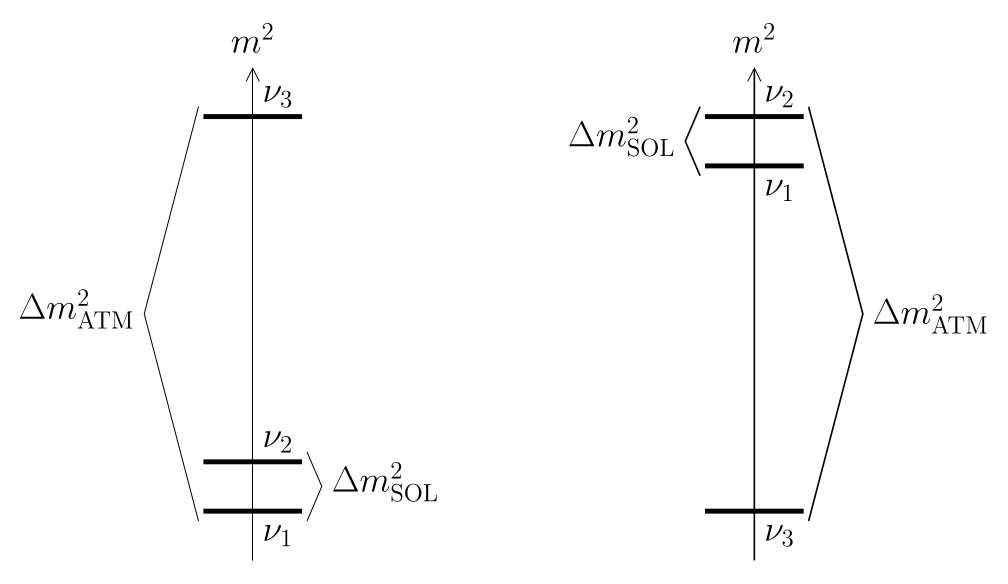
\includegraphics[width=0.85\linewidth]{figures/02_neutrino/Neutrino_mass_hierarchy.png}
    \caption{The two possible neutrino mass hierarchies. Normal ordering is shown on the left and inverted ordering on the right~\cite{giunti_fundamentals_2007}.}
    \label{fig:Neutrino_mass_hierarchy}
\end{figure}

\begin{itemize}
    \item Normal ordering: $m_1 < m_2 \ll m_3$
    \item Inverted ordering: $m_3 \ll m_1 < m_2$
\end{itemize}



\subsection{Neutrinoless double beta decay}
\label{sec:0vbb}

The most promising method to determine whether neutrinos are Dirac or Majorana particles is to search for processes that violate the total lepton number. If such a process is discovered, it would imply that neutrinos are Majorana particles.  
The most sensitive experimental probe for the violation of $L$ is neutrinoless double beta decay, a simultaneous beta decay of two neutrons without emission of neutrinos~\cite{navas_review_2024}. 
Beta decays describe the decay of a neutron into a proton, $(A,Z) \rightarrow (A,Z+1)$ inside a nucleus ($\beta^-$-decay). If $m_{(A, Z+2)} < m_{(A,Z)}$, double beta decay ($2 \nu \beta^- \beta^-$) can occur:

\begin{equation} 
\label{eq:2vbb}
	(A, Z) \rightarrow (A, Z+2) + 2 \, e^- + 2 \, \bar{\nu}_e \,.
\end{equation}

\noindent This is a second-order weak interaction. As such, the decay rate scales as $\Gamma^{2 \nu} \propto G_F^4$, leading to a highly suppressed transition probability. The resulting half-lives are typically of order $T^{2 \nu}_{1/2} \sim 10^{20}$~yr, depending on the nuclear matrix element and available phase space. 
To be experimentally feasible, normal $\beta^{-}$ decay should be energetically forbidden ($m_{(A, Z+1)} > m_{(A, Z)}$)~\cite{zuber_neutrino_2020}. 
Only if neutrinos are Majorana particles, $L$ is not conserved, and neutrinoless double beta decay can occur: 


\begin{equation} 
\label{eq:0vbb}
	(A, Z) \rightarrow (A, Z+2) + 2 \, e^{-} \,.
\end{equation}


\begin{figure}[t]
    \centering
    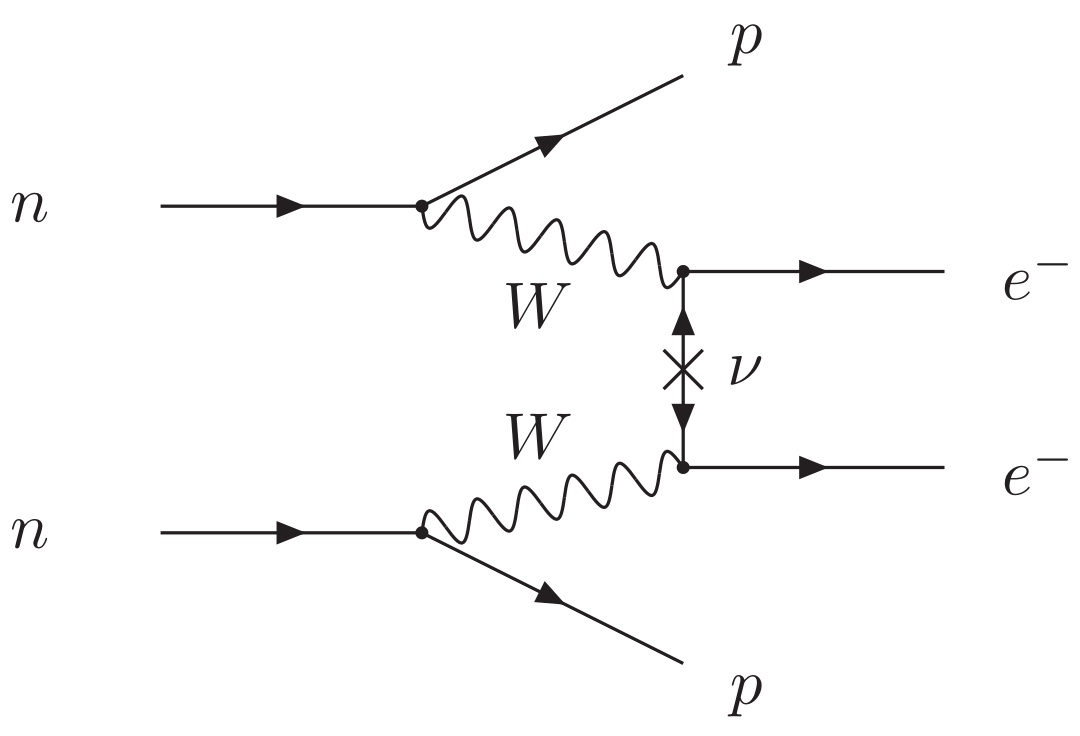
\includegraphics[width=0.75\linewidth]{figures/02_neutrino/feynman_0vbb.png}
    \caption{Feynman diagram of neutrinoless double beta decay: Two neutrons decay into protons and electrons. Only if the neutrino is its own antiparticle, it can be emitted and reabsorbed by a virtual intermediate state, enabling this process~\cite{navas_review_2024}.}
    \label{fig:feynman_0vbb}
\end{figure}


The Feynman diagram for $0 \nu \beta \beta$ decay is shown in figure~\ref{fig:feynman_0vbb} and illustrates why this process is not allowed in the SM: the upper vertex represents $W^{-} \rightarrow e^- + \bar{\nu}_e$ and the lower vertex corresponds to the decay $W^{-} + \nu_e \rightarrow e^-$. Since the exchanged neutrino is emitted as an antineutrino and absorbed as a neutrino, the process is only possible if $\nu_e = \bar{\nu}_e$.

For $0 \nu \beta \beta$ decay, the decay rate $\Gamma^{0 \nu}$ is given by Fermi's golden rule:

\begin{equation} \label{eq:0vbb_halflife}
	\Gamma^{0 \nu} = \frac{\ln 2}{T^{0 \nu}_{1/2}} = \ln 2 \cdot G^{0 \nu}(Q, Z) \cdot \abs{M^{0 \nu}}^2 \cdot \left( \frac{m_{\beta \beta}}{m_e} \right)^2 \,.
\end{equation}

Here, $T^{0 \nu}_{1/2}$ is the half-life, $G^{0 \nu} (Q,Z)$ the phase space factor, and $Q$ the total kinetic energy released. The quantity $M^{0 \nu}$ is the nuclear matrix element, $m_{\beta \beta}$ the effective Majorana mass and $m_e$ the electron mass. The nuclear matrix element $M^{0 \nu}$ carries a model-dependent uncertainty of a factor 2-3~\cite{engel_status_2017}, and the effective Majorana mass is given by:

\begin{equation}
\label{eq:effective_majorana_mass}
    \abs{m_{\beta \beta}} = \abs{\sum_i \mathcal{U}_{ei} ^2m_i} \,
\end{equation}

\noindent where $\mathcal{U}$ is the PMNS matrix and $m_i$ are the mass eigenstates. A full derivation of~\refeq{eq:0vbb_halflife} is presented in~\cite{bilenky_neutrinoless_2015}. 

In this work, we refer to the Q-value of $0 \nu \beta \beta$ decay as $Q_{\beta \beta}$. Furthermore, we define the signal half-rate as

\begin{equation}
\label{eq:signal_half_rate}
    \mathcal{S} = \frac{1}{T^{0 \nu}_{1/2}} \,.
\end{equation}

\noindent This definition of $\mathcal{S}$ corresponds to the half-rate, as it is the inverse of the half-life. This follows the common usage in the field (see~\cite{lnote_25001}, eq.~(8)), where the phase-space factor $G^{0 \nu}$ is defined to include a factor of $1/\ln 2$:

\begin{equation}
\label{eq:0vbb_phase_space}
    G^{0 \nu}(Q,Z) \propto \frac{G_F^4}{\ln 2} \cdot Q_{\beta \beta}^5
\end{equation}


\subsubsection{Experimental searches}

Double beta decay should be observable in 35 isotopes, but due to practical reasons, only 9 are of experimental interest: $^{48}$Ca, $^{76}$Ge, $^{82}$Se, $^{96}$Zr, $^{100}$Mo, $^{116}$Cd, $^{130}$Te, $^{136}$Xe and $^{150}$Nd~\cite{rodejohann_neutrino-less_2011}.
The detection of (neutrinoless) double beta decay is characterized by measuring the kinematic parameters of the emitted electrons~\cite{dolinski_neutrinoless_2019}. 
In the case of $0 \nu \beta \beta$ decay, the total energy carried by the emitted electrons equals the Q-value of the decay (neglecting nuclear recoil), resulting in a monoenergetic peak. 
In practice, this peak is broadened due to the finite energy resolution of the detector. In contrast, $2 \nu \beta \beta$ decay produces a continuous energy spectrum, as the undetected neutrinos carry away varying amounts of energy. 
Figure~\ref{fig:expected_energy_spec} illustrates the expected energy depositions for both decay modes in the transition $^{76} \mathrm{Ge} \rightarrow \, ^{76} \mathrm{Se}$.
The Q-value for this process is $Q_{\beta \beta} = 2039.0612 \pm 0.0075$~keV~\cite{Huang_2021}.

\begin{figure}
    \centering
    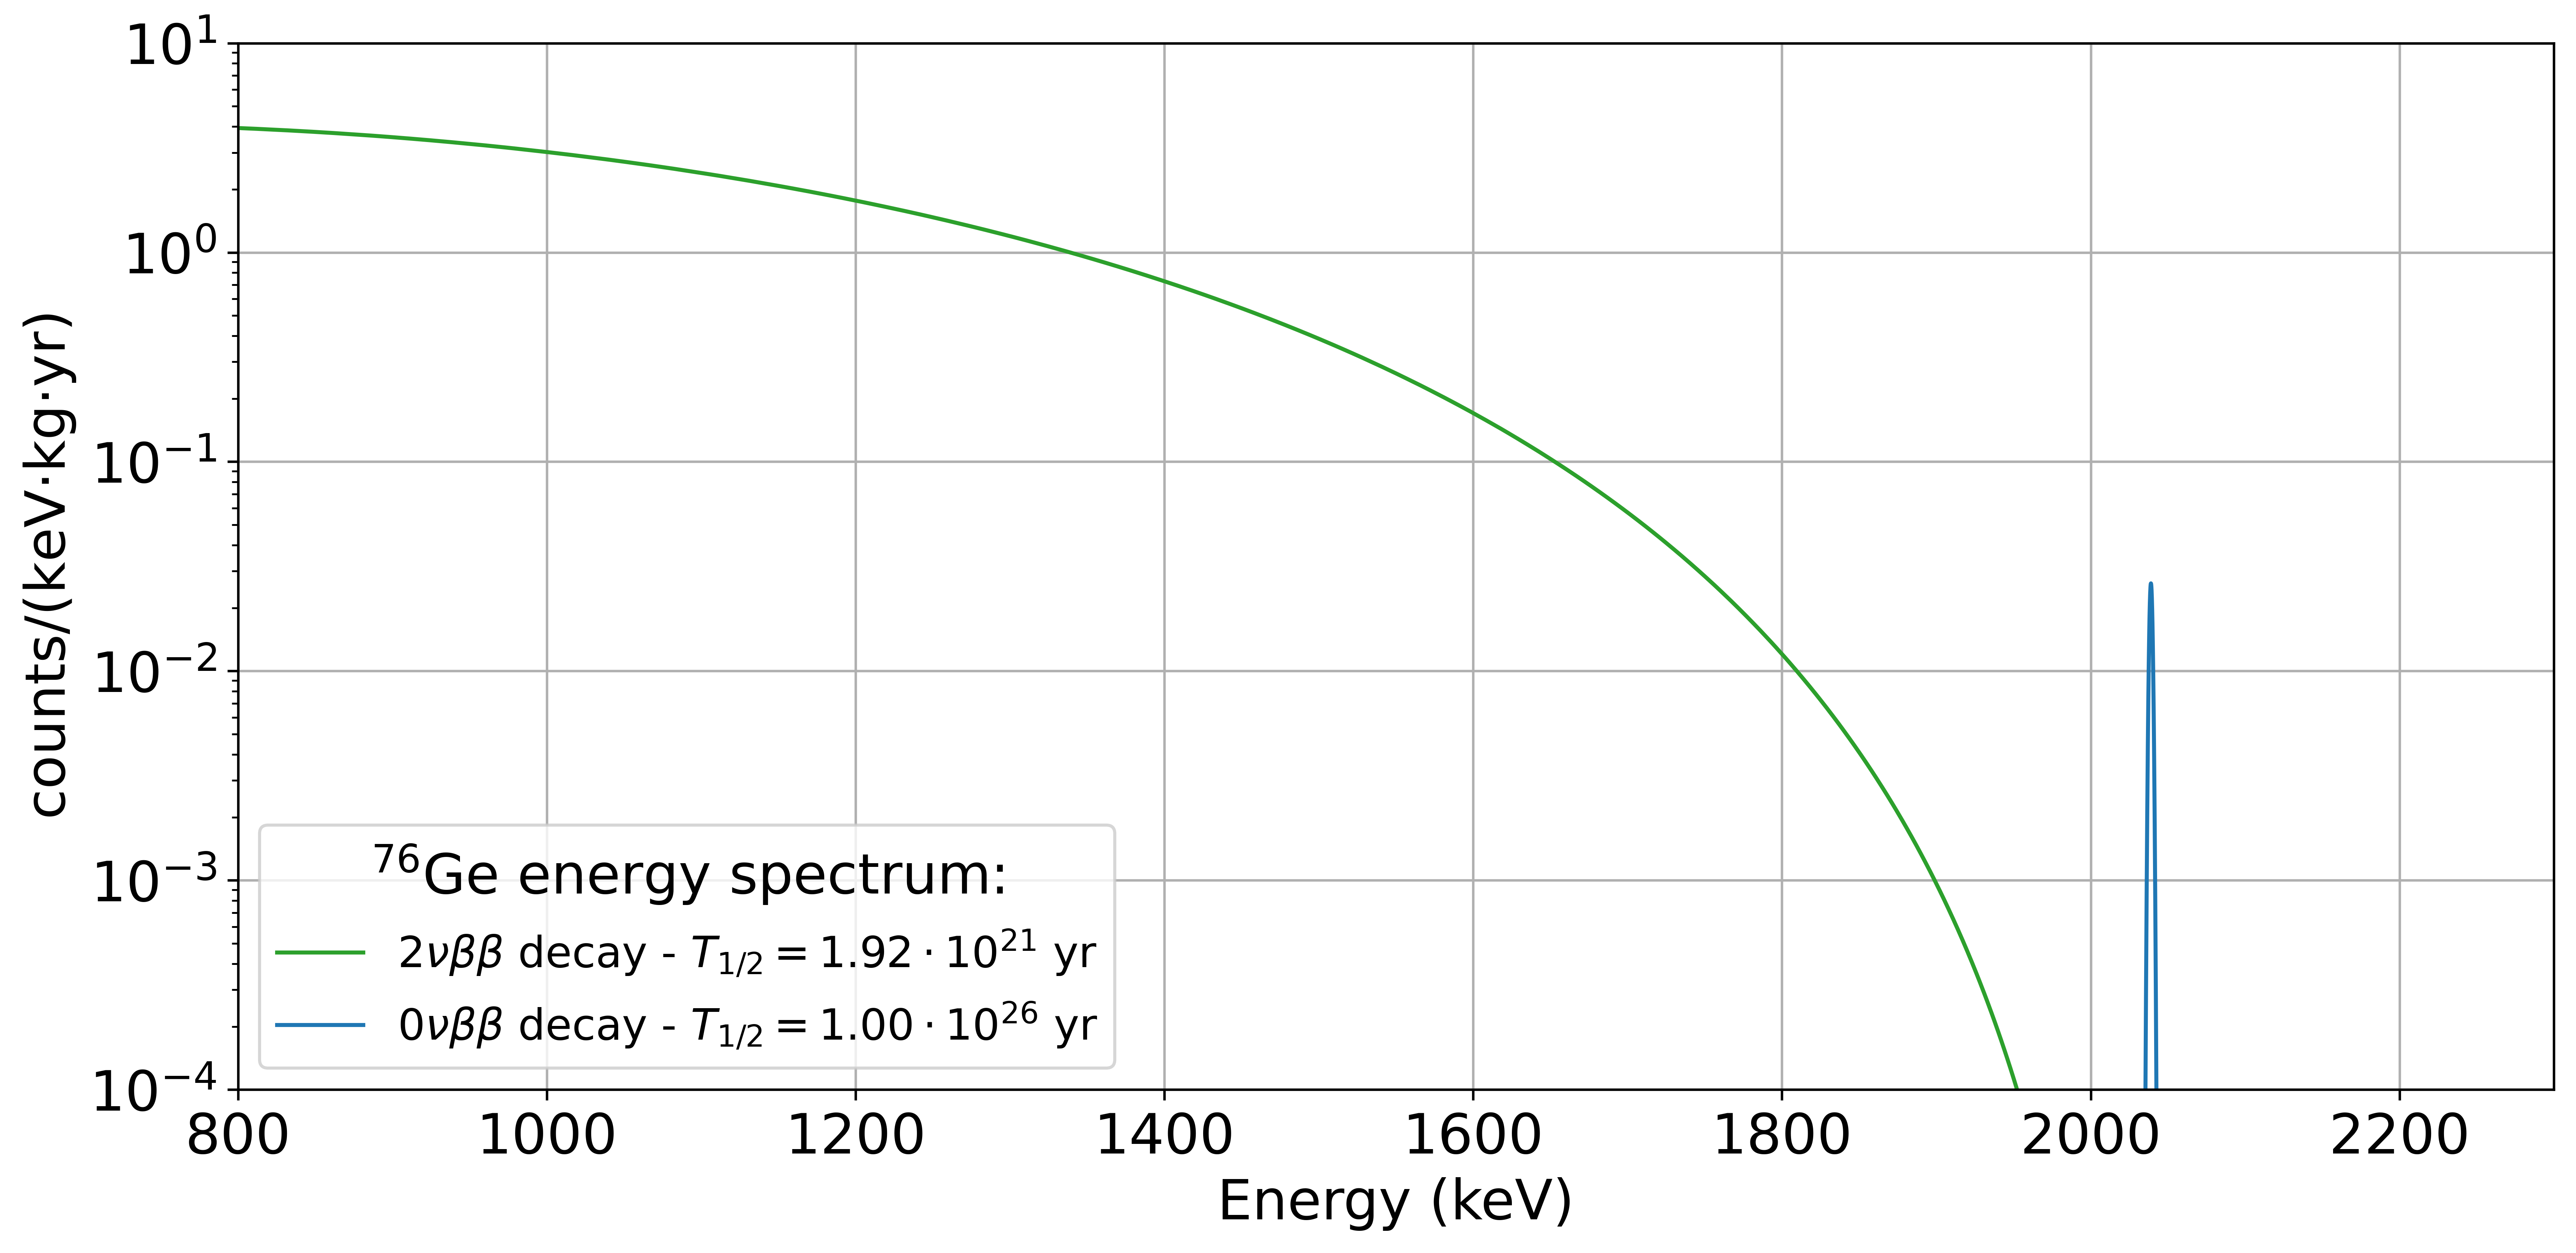
\includegraphics[width=0.95\linewidth]{figures/02_neutrino/Energyspectrum_Ge76.png}
    \caption{Expected energy spectra for $2 \nu \beta \beta$ and $0 \nu \beta \beta$ decay in $^{76}$Ge. The $2 \nu \beta \beta$ decay spectrum is computed using the phase space distribution from \cite{kotila_phasespace_2012}, scaled to a half-life of $1.92 \cdot 10^{21}$~yr. The $0 \nu \beta \beta$ decay signal is modeled as a Gaussian at $Q_{\beta \beta} = 2039$~keV, assuming a detector resolution of FWHM~$= 2.5$~keV and a half-life of $10^{26}$~yr, following the estimates from the GERDA collaboration~\cite{dandrea_neutrinoless_2021}.}
    \label{fig:expected_energy_spec}
\end{figure}


The sensitivity to the half-life depends heavily on the amount of background: 

\begin{equation}
\label{eq:0vbb_hl_sensitivity}
	T^{0 \nu}_{1/2} \propto 
    \begin{cases}
        a \cdot M \cdot \epsilon \cdot t &  \text{background free} \\
        a \cdot \epsilon \cdot \sqrt{\frac{M \cdot t}{B \cdot \Delta E}} &  \text{with background}
    \end{cases}    
\end{equation}

\noindent Here, $a$ is the isotopic abundance, $\epsilon$ the efficiency of the detection, $M$ the total mass used in kg, $t$ the time measured in years, $B$ the background in counts/(keV$\cdot$kg$\cdot$yr), and $\Delta E$ is the energy resolution in keV~\cite{zuber_neutrino_2020, dolinski_neutrinoless_2019}. 
Equation~\refeq{eq:0vbb_hl_sensitivity} shows why it is of utmost importance to achieve a quasi-free background: If there are many background events, the sensitivity scales $(M \cdot t)^{1/2}$ instead of $M \cdot t$. Moreover, the energy resolution must be sufficiently good, otherwise the sharp peak at $Q_{\beta \beta}$ is indistinguishable from the $2 \nu \beta \beta$ decay tail~\cite{delloro_neutrinoless_2016}. 

Neutrinoless double beta decay has not been observed yet. However, several different experiments can constrain the $0 \nu \beta \beta$ decay half-life: 
The KamLAND-Zen consists of a tank filled with a liquid scintillator that contains a balloon of Xenon-loaded liquid scintillator as the $0 \nu \beta \beta$ decay source. Inside the tank are almost 2000 PMTs alongside the walls. KamLAND-Zen achieved $T^{0 \nu}_{1/2} > 2.3 \times 10^{26}$yr with $^{136}$Xe~\cite{kamland-zen_collaboration_search_2023}. 

The CUORE experiment is a cryogenic calorimeter that consists of 988 TeO$_2$ crystals. Energy depositions in the crystals will lead to a temperature rise, which is transformed into an electrical signal. The experiment measured a half-life of $T^{0 \nu}_{1/2} > 2.2 \times 10^{25}$yr using over 200~kg of $^{130}$Te~\cite{adams_search_2022}. Reported values are at $90 \% $ C.L. 

CUPID-Mo, which served as a demonstrator for the upgrade of CUORE, contains enriched Li$_2$MoO$_4$ scintillating calorimeters, obtaining a half-life of $T^{0 \nu}_{1/2} > 1.8 \times 10^{24}$ for $^{100}$Mo~\cite{augier_final_2022}. 


A very promising approach is ionizing radiation detection, as shown by the GERDA and MAJORANA DEMONSTRATOR (MJD) experiments. While not exclusively to these setups, both experiments showed that a HPGe-based approach is highly efficient in terms of energy resolution and intrinsic background suppression due to the detector-source identity~\cite{dandrea_neutrinoless_2021}. 
The GERDA collaboration achieved an unprecedentedly low background of $5.2 \times 10^{-5}$ counts/(keV$\cdot$kg$\cdot$yr) and an exposure-weighted energy resolution of $(2.9 \pm 0.1)$~keV full width half maximum (FWHM) at $Q_{\beta \beta}$ for the detector geometry used in this work
. The final value reported by the GERDA collaboration was $T^{0 \nu}_{1/2} > 1.8 \times 10^{26}$yr at $90\%$ C.L.~\cite{gerda_collaboration_final_2020}.  
MJD reached an impressive energy resolution of $(2.55 \pm 0.09)$~keV FWHM at $Q_{\beta \beta}$, with a final half-life of $T^{0 \nu}_{1/2} > 8.3 \times 10^{25}$ yr at $90 \%$ C.L.~\cite{majorana_collaboration_final_2023}.

In addition to direct searches, complementary constraints on the absolute neutrino mass scale arise from cosmological observations and kinematic measurements. 
The Planck satellite has placed an upper limit on the sum of neutrino masses, currently constrained to $\sum m_\nu < 0.16$~eV at 95\% confidence level under the $\Lambda \mathrm{CDM}$ model~\cite{ivanov_cosmological_2020}. 

On the experimental side, the KATRIN experiment probes the kinematic endpoint of tritium beta decay, directly measuring the effective electron neutrino mass: $m_\nu = \sqrt{\sum \abs{U_{ei}}^2 \, m_i^2}$. Its latest results set an upper limit of $m_{\nu} < 0.8 \,\mathrm{eV} c^{-2}$ at 90\% CL~\cite{aker_direct_2022}.
While not sensitive to the Majorana or Dirac nature, this result further constrains the possible values of $m_{\beta \beta}$, especially in the case of inverted mass ordering. 



\subsection{Current challenges and future prospects}


Assuming three neutrinos, oscillation experiments constrain six parameters: Two mass differences, three mixing angles, and a CP-violating phase. A global analysis of neutrino oscillation data, such as provided by the NuFIT collaboration, yields ever-tighter bounds on these parameters~\cite{esteban_nufit-60_2024}. 

However, oscillation experiments are insensitive to the absolute neutrino mass scale. In this regard, cosmological observation provides a complementary probe: Relic neutrinos affect the large-scale structure of the universe and leave an imprint on the cosmic microwave background through their contribution to the total energy density. 
To determine the neutrino mass hierarchy, neutrinoless double beta decay experiments remain a promising approach, as the measured half-life can be translated into upper limits on the effective Majorana mass -- assuming that the decay is dominated by the exchange of light Majorana neutrinos~\cite{gerda_collaboration_final_2020}.
The sensitivity difference between normal and inverted ordering arises because in the latter case, the two heaviest neutrino mass eigenstates contribute significantly to $m_{\beta \beta}$, leading to a non-zero lower bound. 

For normal ordering, destructive interference between the contributions from the three mass eigenstates can suppress $m_{\beta \beta}$ values close to zero, potentially beyond the reach of upcoming experiments. 
Current limits include $m_{\beta \beta} < 79-180$~meV from GERDA and $m_{\beta \beta} < 36-156$~meV from KamLAND-Zen~\cite{gerda_collaboration_final_2020, abbasi_measurement_2023}. The relatively large range in values reflects uncertainties in the nuclear matrix element involved in the decay process.  

Figure~\ref{fig:Lobster_2024} shows the allowed regions for the effective Majorana masses $m_{\beta \beta}$ as a function of the lightest neutrino mass $m_{\mathrm{min}}$, for both normal and inverted mass ordering. For the inverted hierarchy, next-generation $0 \nu \beta \beta$ decay experiments such as SNO$+$ (using Cherenkov detectors), NEXT (a xenon time projection chamber), or LEGEND (using HPGe detectors) are expected to reach sensitivities that fully probe the relevant parameter space~\cite{agostini_discovery_2017}. \\
Among these, the LEGEND experiment stands out for its combination of excellent energy resolution, ultra-low background techniques and scalability. With its staged approach from LEGEND-200 to LEGEND-1000, the experiment is designed to explore half-lives beyond $10^{28}$ years and approach the full coverage of inverted ordering. 
The next chapter introduces the LEGEND experiment in detail, with an emphasis on the detector technology. 

\begin{figure}
    \centering
    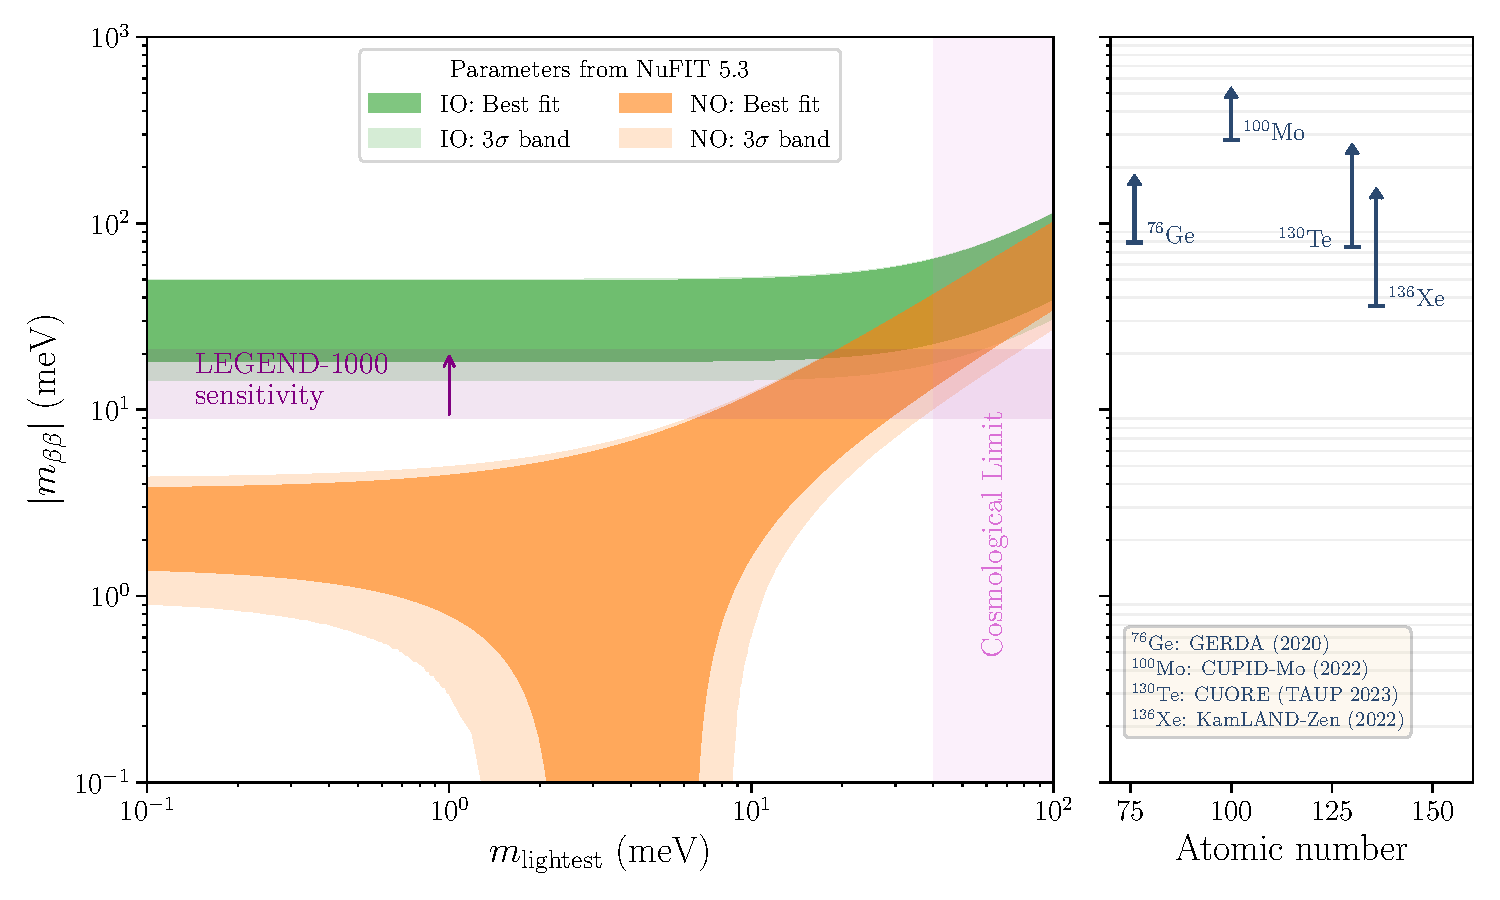
\includegraphics[width=1\linewidth]{figures/02_neutrino/Lobster_plot_NuFIT_5-2.pdf}
    \caption{Left: Effective Majorana mass $m_{\beta \beta}$ for inverted and normal ordering as a function of the lightest neutrino mass $m_\mathrm{min}$, including the projected sensitivity of the LEGEND-1000 experiment. Right: Effective Majorana masses obtained for different isotopes. The figure is created with code from~\cite{torres_toej93lobsterplot_2024}.}
    \label{fig:Lobster_2024}
\end{figure}
